\documentclass{ximera}
%% You can put user macros here
%% However, you cannot make new environments

\listfiles

\graphicspath{{./}{firstExample/}{secondExample/}}

\usepackage{tikz}
\usepackage{tkz-euclide}
\usepackage{tikz-3dplot}
\usepackage{tikz-cd}
\usetikzlibrary{shapes.geometric}
\usetikzlibrary{arrows}
%\usetkzobj{all}
\pgfplotsset{compat=1.13} % prevents compile error.

%\renewcommand{\vec}[1]{\mathbf{#1}}
\renewcommand{\vec}{\mathbf}
\newcommand{\RR}{\mathbb{R}}
\newcommand{\dfn}{\textit}
\newcommand{\dotp}{\cdot}
\newcommand{\id}{\text{id}}
\newcommand\norm[1]{\left\lVert#1\right\rVert}
 
\newtheorem{general}{Generalization}
\newtheorem{initprob}{Exploration Problem}

\tikzstyle geometryDiagrams=[ultra thick,color=blue!50!black]

%\DefineVerbatimEnvironment{octave}{Verbatim}{numbers=left,frame=lines,label=Octave,labelposition=topline}



\usepackage{mathtools}


\title{How to Use this Text} \license{CC BY-NC-SA 4.0}



\begin{document}
\begin{abstract}
\end{abstract}
\maketitle



\section*{How to Use this Text}
In this section we will cover some technical aspects of using this text.  In particular, you will learn about the following features:
\begin{itemize}
    \item Machine-graded exercises.
    \item Using GeoGebra interactives.
    \item Using Octave cells.
\end{itemize}

\subsection*{Machine-Graded Exercises}
Machine-graded exercises on the XIMERA platform are designed to help you learn without penalizing you for not getting the right answer the first time.  You can enter answers until you get it right.  
\begin{question}
Try typing $5$ in the answer cell below, then answer the question correctly.
\begin{hint}
    The answer is SMALLER than 5.
\end{hint}
$$2+2=\answer{4}$$
\end{question}
You can enter answers in fraction or in decimal form, as long as your answers are exact.  For example, the following answers are considered equivalent: $\frac{10}{4}=\frac{5}{2}=2.5$.  However, $\frac{1}{3}\neq 0.333$.

\subsection*{GeoGebra Interactives}
GeoGebra interactives are one of the most exciting features of this text.  They are designed to give you valuable geometric insights by helping you interact with mathematical objects in three dimensions, and by letting you animate processes.  For example, you can visualize two planes and a point in $\RR^3$ by rotating the following figure.  RIGHT-CLICK and DRAG to rotate the figure for a better view.  Try it!

\begin{center}
\geogebra{unceva9g}{900}{600}
\end{center}

The following screenshot highlights the \dfn{navigation bar} and the \dfn{slider}.  Both tools are used to guide you through constructions and algorithms, one step at a time.  Start by using the \dfn{navigation bar}.  Click the arrows to advance slides.  When the \dfn{slider} appears, you can use it to animate the perpendicular vector.
\begin{image}
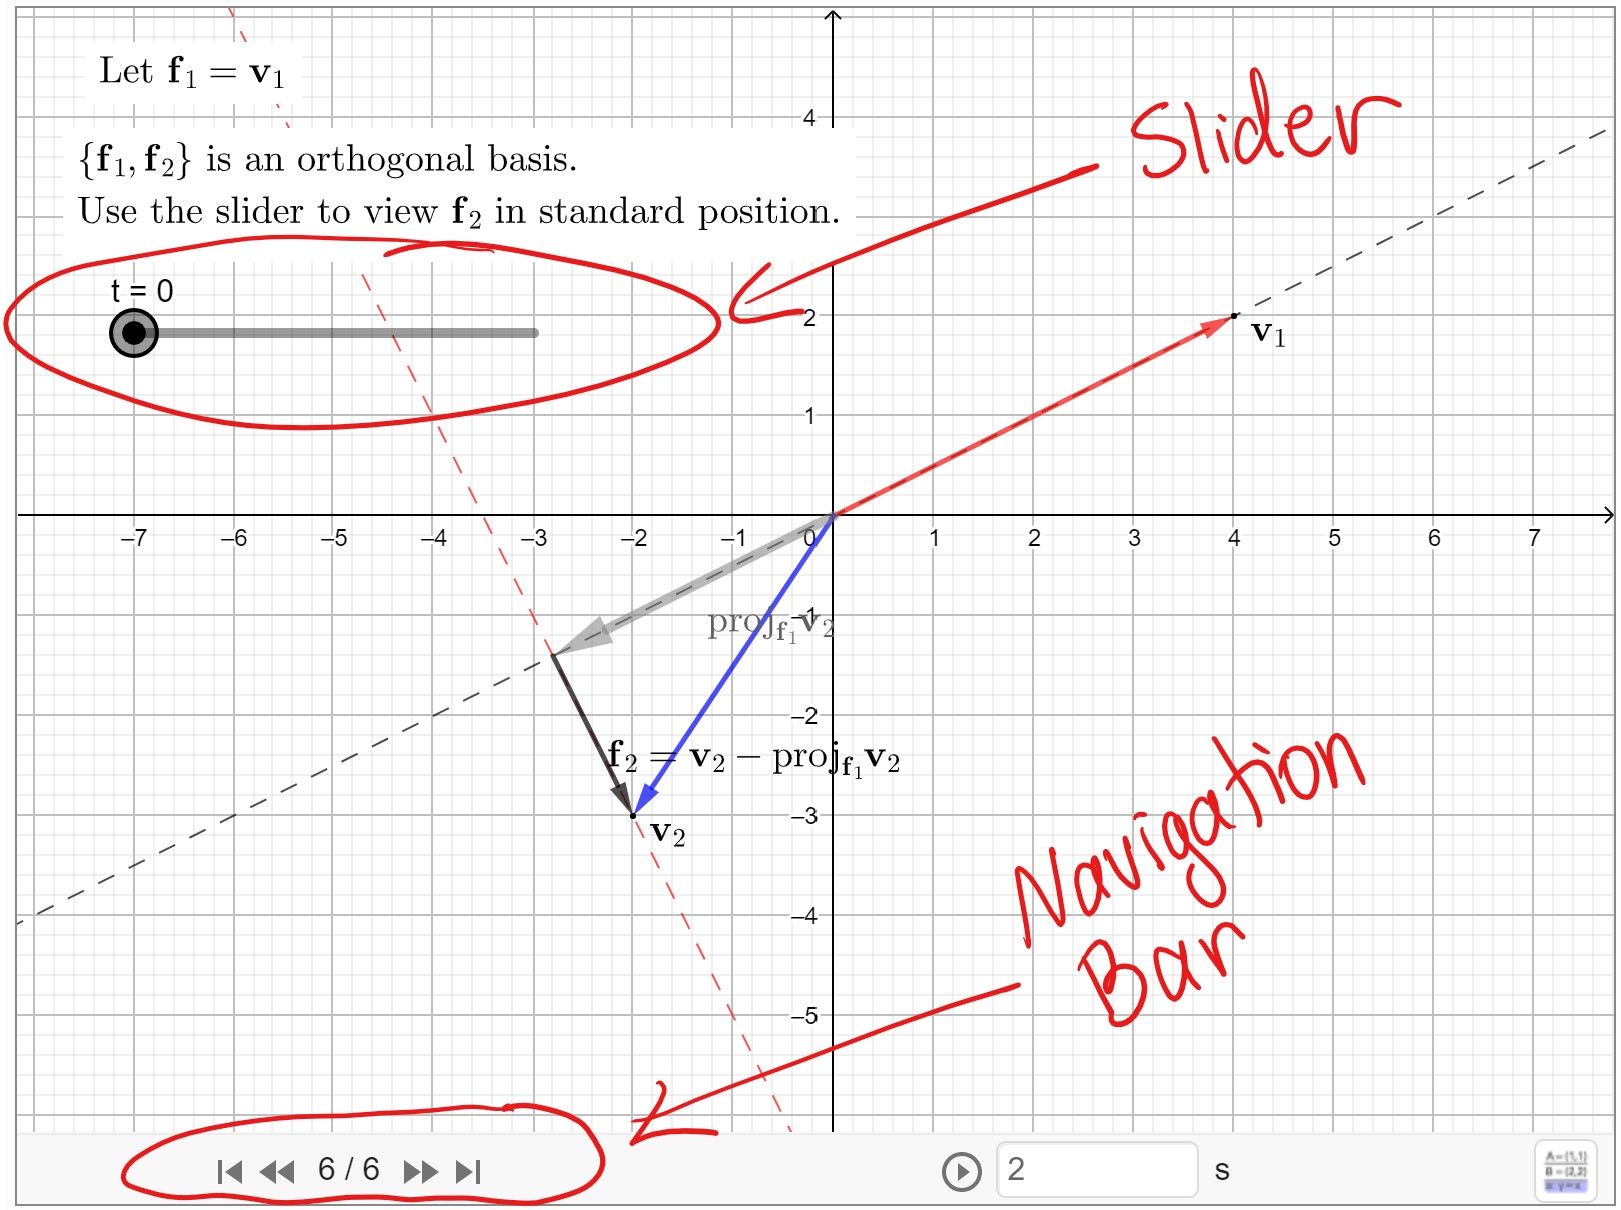
\includegraphics{GeoGebraScreenshot1.jpg}
\end{image}
Try it out below:
\begin{center}
\geogebra{xtqppyav}{800}{600}
\end{center}
GeoGebra offers many more features.  Make sure to read the directions in each interactive!

\subsection*{Octave Cells}
Please refer to the \href{https://ximera.osu.edu/linearalgebradzv3/xOctave}{Octave Tutorial} for more information on how to use Octave and Octave Cells.

\subsection*{Keeping Track of Progress}
XIMERA does not require a log-in.  Your answers will be saved automatically, and XIMERA will remember your progress.  \begin{warning}
    You will lose your work if you clear out your cookies.  You will also lose your work if you switch to a different computer.
\end{warning}

Instructors may require that students submit a proof of completion.  This is easy to do. 
\begin{itemize}
    \item Go to the landing page for the course.
    \begin{image}
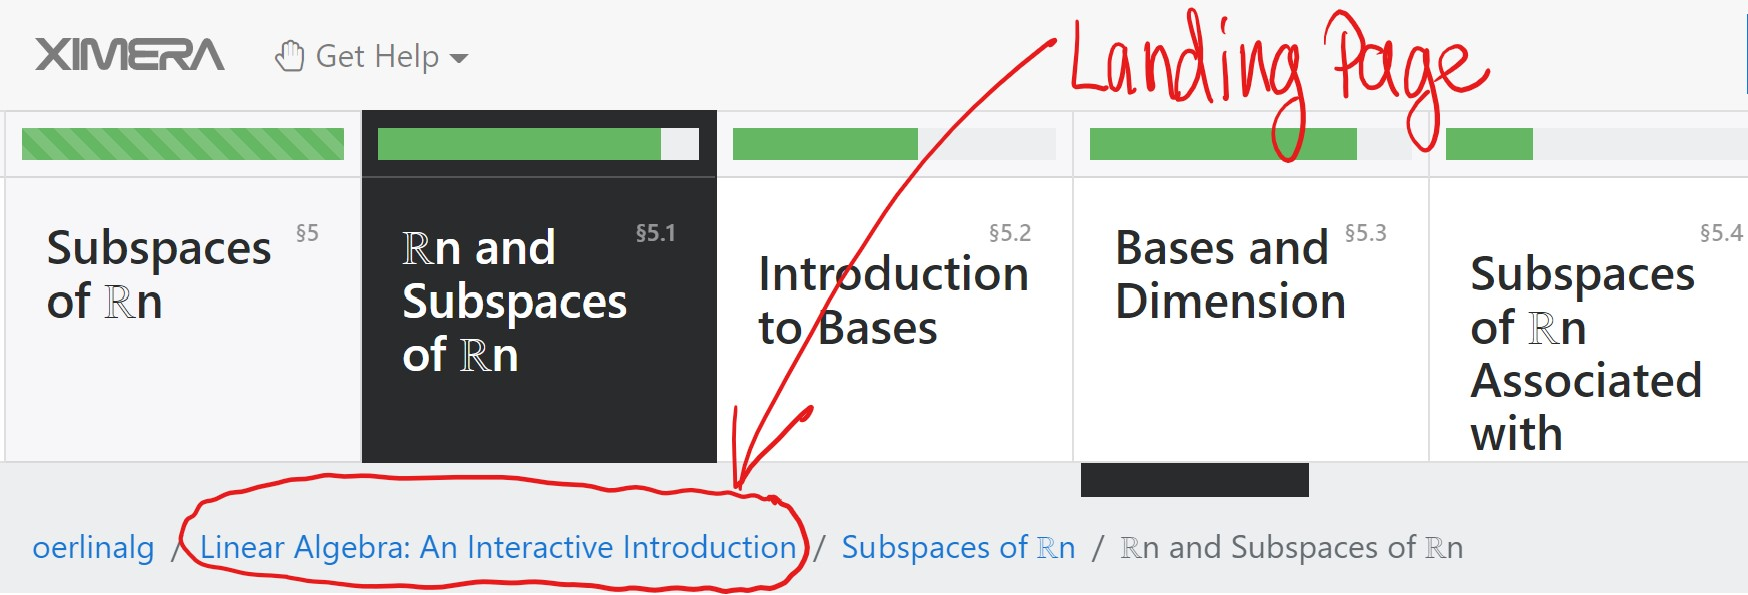
\includegraphics{ximeraScreenshot1.jpg}
\end{image}
\item Scroll to the bottom of the page and click on the Certificate button.
\begin{image}
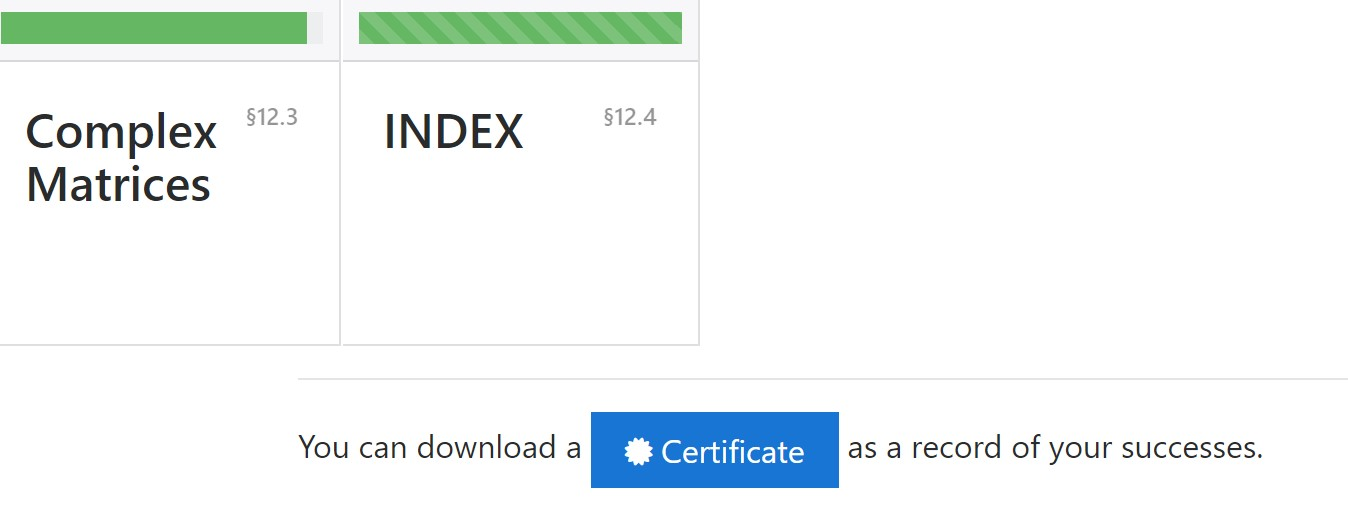
\includegraphics{ximeraScreenshot2.jpg}
\end{image}
\item
Your instructor may ask you to submit a screenshot of your completion summary.
\begin{image}
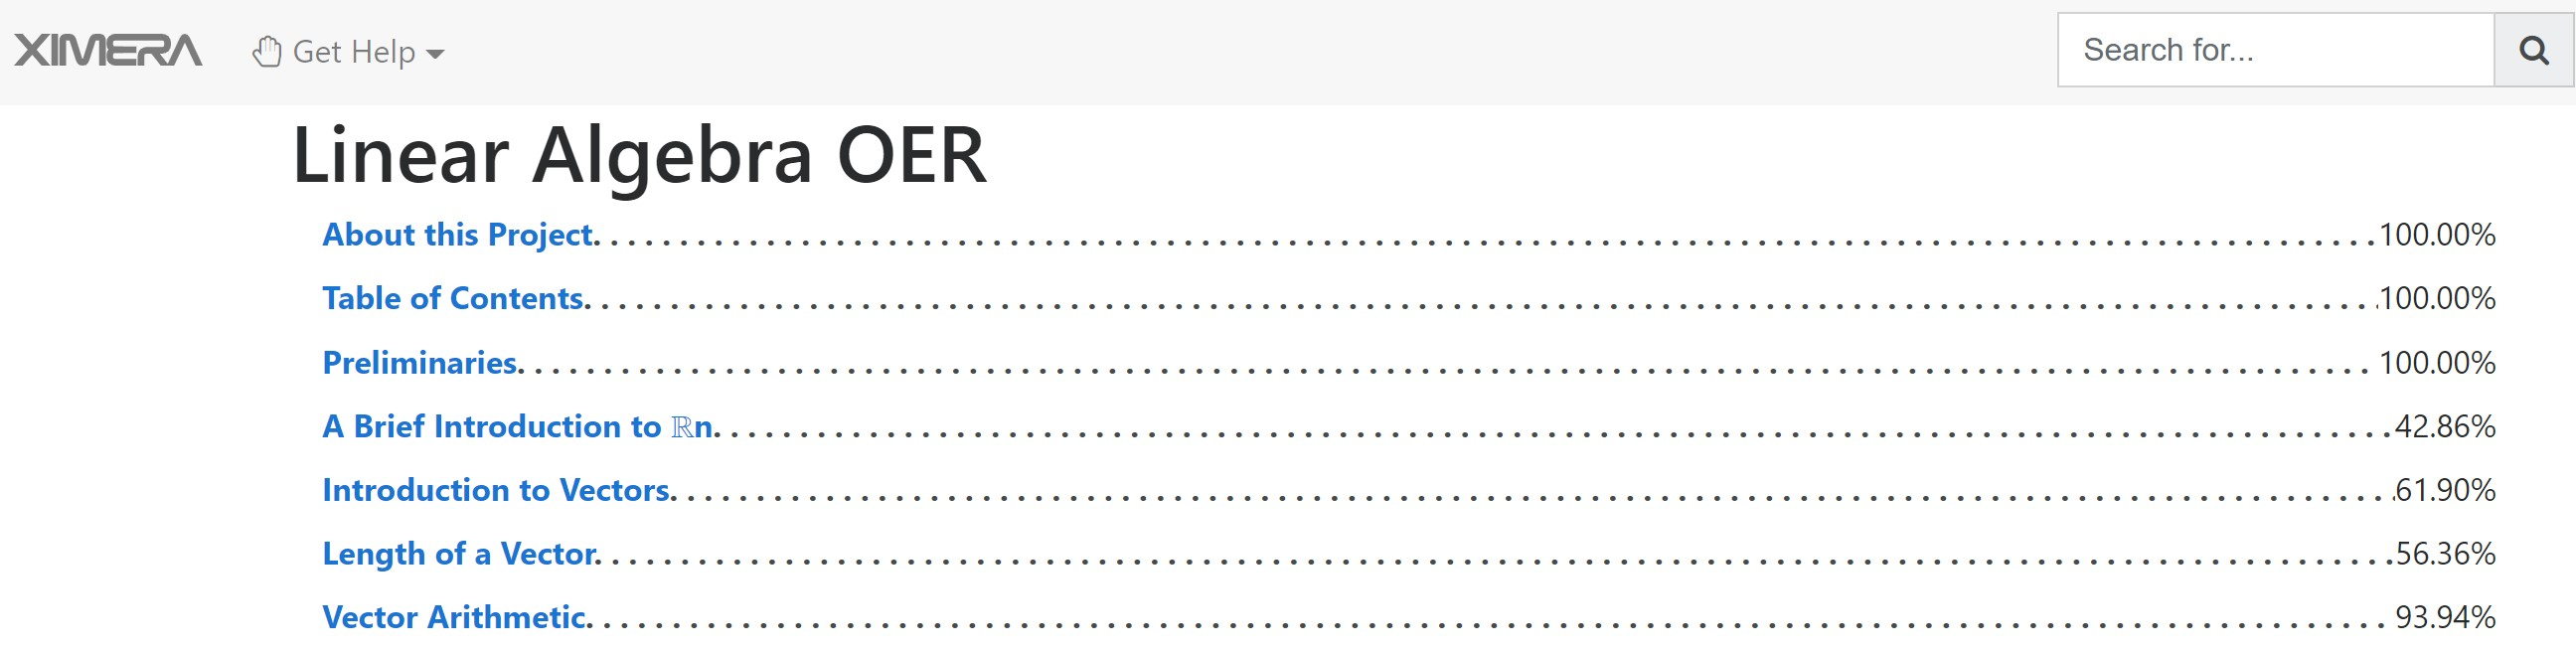
\includegraphics{ximeraScreenshot3.jpg}
\end{image}
\end{itemize}
% \subsection*{Data Collection and Usage}
% Event stream data from user interactions with the platform -- such as mouse clicks, and submitted answers -- are stored on a secure server at the Ohio State University.  There is no plaintext storage of passwords, and only encrypted protocols for authentication are used.  Anonymized event log is available to the authors of this text through secure access requiring a private key. (GPG is used for this.)   Event log data may be used for research purposes and to improve the product.
\end{document}
